% !TEX root = mythesis.tex

%==============================================================================
\chapter{Data Analysis}
\label{sec:data_analysis}
%==============================================================================
\section{Image Inspection}
%
For a clearer visualization of the emission structures, a contour plot of the corrected wavelet-filtered image is presented (Figure \ref{fig:contour_wvl_filtered}). The group exhibits a spherically symmetrical appearance, with a distinct emission boundary clearly visible at \(R_{500}\). Furthermore, emission beyond \(R_{500}\) and \(R_{200}\) is difficult to distinguish from the complex background. A noticeable asymmetry is observed in the background emission, with a drop-off to the north compared to the south. 
\begin{figure}[htbp]
    \centering
    \includegraphics[width=\textwidth]{data_analysis/wvl_filtered_contour.pdf}
    \caption{
        Contour plot of the corrected wavelet-filtered image. The colorbar represents counts per second. A distinct emission cut is visible at \(R_{500}\), while the emission beyond \(R_{500}\) is diffcult to discern from the background.}
    \label{fig:contour_wvl_filtered}
\end{figure}
\section{Surface Brightness Analysis}
\subsection{Full Azimuthal Surface Brightness}
To more accurately identify or exclude potential deviations from spherical symmetry, surface brightness analysis will be performed. First, the emission center is estimated by constructing a \(2'\) aperture around the apparent center, as given in Section X. This aperture size is chosen to capture a statistically significant number of photons without leaving the group center. The flux-weighted average of the image coordinates within this aperture yields a right ascension of \SI{64.909}{\degree} and a declination of \SI{2.414}{\degree}. Concentric Anulli of \(1'\) width are constructed from the calculated flux-weighted surface brightness of the group up to to an angular distance of \(80' \sim 1.5R_{200}\). The counts \(C\) within each annulus are determined using the \texttt{funcnts} task from the \texttt{funtools} software, with a Poisson error of \(\sqrt{C}\). The surface brightness \(S\) for each annulus is calculated by
\begin{align*}
    S = \frac{C_\text{image} - C_\text{PIB}}{C_\text{expmap}\cdot A},
\end{align*}
where \(C\) denotes the counts in the photon image, total PIB map, and exposure map, respectively. Errors are calculated using Gaussian error propagation. Furthermore, background estimation is performed using \(10\) circular regions with a \(48'\) radius, each centered \(160'\) from the calculated center of NGC 1550. The average background surface brightness is evaluated for all circles combined and separately for the northern (Circles 1-5) and southern region (Circles 6-10) to account for the possibly significant background gradient. Table \ref{tab:background} lists the average background for all 3 cases. As is clear from the table, all background values consist with each other within a \(1\sigma\)-Intervall. Thus, for the following analysis and interpretation, the total background value obtained from all circles is utilized. 
\begin{figure}[htbp]
    \centering
    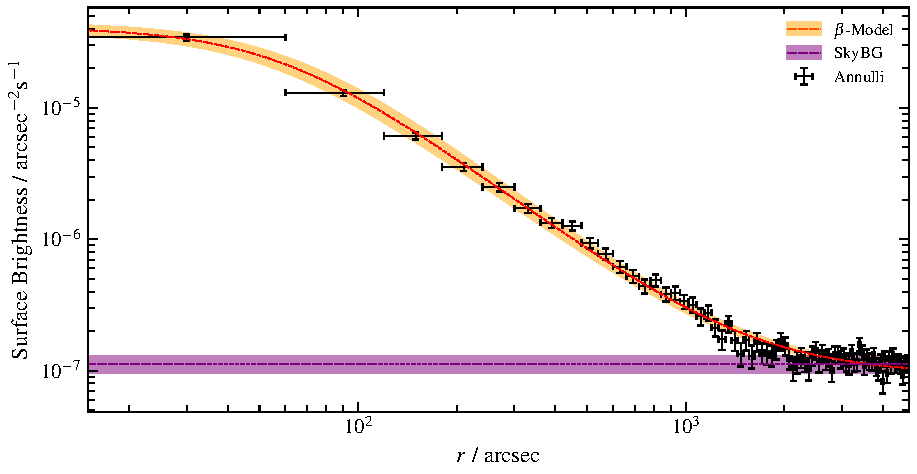
\includegraphics{data_analysis/beta_motel_tot_surf_bri_anulli1_1arcmin.pdf}
    \caption{Surface Brightness within each annulus (black crosses) as a function of distance from the determined SB-center. The dashed orange line represents the best \(\beta\)-model fit, while the purple line indicates the observationally determined background. The shaded regions correspond to their respective \(1\sigma\) intervals.}
    \label{fig:tot_azimuthal_beta_model}
\end{figure}
\begin{table}[htbp]
    \centering
    \begin{tabular}{lcc}
        \toprule
        Region & Background (cts s$^{-1}$ arcsec$^{-2}$) \\
        \midrule
        Southern Background & $13 \times 10^{-8} \pm 2.0 \times 10^{-9}$ \\
        Northern Background & $9.9 \times 10^{-8} \pm 1.2 \times 10^{-8}$ \\
        Total Background    & $11 \times 10^{-8} \pm 1.7 \times 10^{-8}$ \\
        \bottomrule
    \end{tabular}
    \caption{Average background surface brightness for southern, northern, and total regions in units of counts per second per square arcsecond (cts s$^{-1}$ arcsec$^{-2}$).}
    \label{tab:background}
\end{table}
A \(\beta\)-Model is employed to characterize the surface brightness profile, given by
\begin{align*}
    S(r) = S_0 \left(1 + \left(\frac{r}{r_c}\right)^2\right)^{-3\beta + 0.5} + d
\end{align*}
where \(d\) represents the background level. The center of each annulus is taken to be \(r\) and the corresponding surface brightness values are utilized. The optimized parameters and \(\chi^2 / \text{d.o.f}\) (Chi squared per degrees of freedom) are listed in Table \ref{table:full_az_fit_parameters}. Figure \ref{fig:tot_azimuthal_beta_model} illustrates the surface brightness as a function of radial distance from the center, including both the fitted \(\beta\)-Model and the observationally estimated background level.
\begin{table}[h!]
    \centering
    \begin{tabular}{lcccc}
    \toprule
    Parameter & $S_0$ & $\beta$ & $r_c$ & $d$ \\
    \midrule
        & $(4.1 \pm 0.4) \times 10^{-5}$ & $0.478 \pm 0.008$ & $60 \pm 5$ & $(9.3 \pm 0.4) \times 10^{-8}$ \\
    \midrule
    \(\chi^2 / \text{d. o. f}\) & \multicolumn{4}{c}{0.96} \\
    \bottomrule
    \end{tabular}
    \caption{Fit parameters, their errors, and the reduced chi-squared value.}
    \label{table:full_az_fit_parameters}
\end{table}
As one can clearly see from \ref{fig:tot_azimuthal_beta_model} and the \(\chi^2/\text{d.o.f}\) value of \(0.96\), the beta model describes the surface brightness profile well and a value of \(\beta = \num{0.478\pm0.008}\) is obtained. This is consist with the findings of THE ALMIGHTY FLYING SPAGHETTI MONSTER.The estimated and fitted backgrounds are consistent. A two-beta model fit, however, was not successful. This can be attributed to the limited angular resolution in the core region and the degeneracy between the core radius and \(\beta\).
\subsection{Beta Model and Residual Image}
Using the parameters from Table \ref{tab:background}, a beta model image (Fig. \ref{fig:beta_model}) and a residual image (Fig. \ref{fig:residual_image}) are created. The beta model image is generated by distributing the one-dimensional beta model across the image. This involves computing the distance from the surface brightness center to each coordinate \((x, y)\) in the image and then scalling the output of the beta model by the eROSITA pixel area of \(16\text{arcsec}^2\). The residual image was obtained by subtracting the scaled beta model from the fully corrected image:
\begin{align*}
    \text{res. img}(x, y) = \text{corr. img}(x, y) - S(\sqrt{x^2 + y^2}) \cdot \text{pix. area}
\end{align*}
The residual image reveals that, except at the very center of the galaxy group, the beta model slightly overestimates the emission around the core. This overestimation can be attributed to the absence of a second beta component, as a single beta model often inadequately describes the inner core emission, leading to higher-than-expected values.
\begin{figure}[htbp]
    \centering
    \begin{subfigure}[b]{0.48\textwidth}
        \centering
        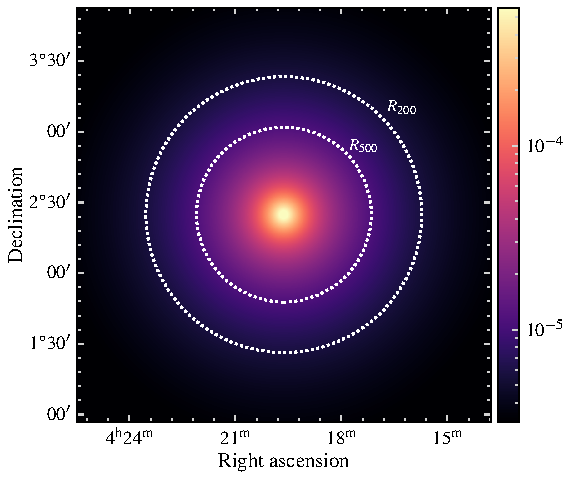
\includegraphics[width=\textwidth]{data_analysis/beta_model.pdf}
        \caption{Beta model image}
        \label{fig:beta_model}
    \end{subfigure}
    \hfill
    \begin{subfigure}[b]{0.48\textwidth}
        \centering
        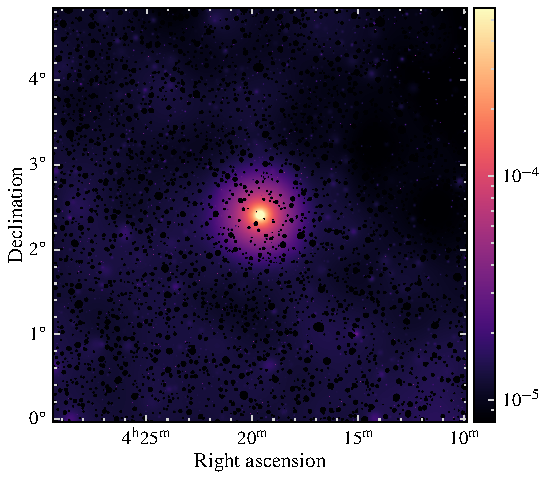
\includegraphics[width=\textwidth]{data_reduction/wlt_filtered_cheese.pdf}
        \caption{Residual image}
        \label{fig:residual_image}
    \end{subfigure}
    \caption{Comparison of the beta model image and the residual image. The colorbar indicates counts per second. The residual image indicate that the beta model slightly overestimates the emission around the core, likely due to the inadequacy of a single beta model in capturing the core's emission.}
    \label{fig:comparison_beta_residual}
\end{figure}
